\documentclass[1p]{elsarticle_modified}
%\bibliographystyle{elsarticle-num}

%\usepackage[colorlinks]{hyperref}
%\usepackage{abbrmath_seonhwa} %\Abb, \Ascr, \Acal ,\Abf, \Afrak
\usepackage{amsfonts}
\usepackage{amssymb}
\usepackage{amsmath}
\usepackage{amsthm}
\usepackage{scalefnt}
\usepackage{amsbsy}
\usepackage{kotex}
\usepackage{caption}
\usepackage{subfig}
\usepackage{color}
\usepackage{graphicx}
\usepackage{xcolor} %% white, black, red, green, blue, cyan, magenta, yellow
\usepackage{float}
\usepackage{setspace}
\usepackage{hyperref}

\usepackage{tikz}
\usetikzlibrary{arrows}

\usepackage{multirow}
\usepackage{array} % fixed length table
\usepackage{hhline}

%%%%%%%%%%%%%%%%%%%%%
\makeatletter
\renewcommand*\env@matrix[1][\arraystretch]{%
	\edef\arraystretch{#1}%
	\hskip -\arraycolsep
	\let\@ifnextchar\new@ifnextchar
	\array{*\c@MaxMatrixCols c}}
\makeatother %https://tex.stackexchange.com/questions/14071/how-can-i-increase-the-line-spacing-in-a-matrix
%%%%%%%%%%%%%%%

\usepackage[normalem]{ulem}

\newcommand{\msout}[1]{\ifmmode\text{\sout{\ensuremath{#1}}}\else\sout{#1}\fi}
%SOURCE: \msout is \stkout macro in https://tex.stackexchange.com/questions/20609/strikeout-in-math-mode

\newcommand{\cancel}[1]{
	\ifmmode
	{\color{red}\msout{#1}}
	\else
	{\color{red}\sout{#1}}
	\fi
}

\newcommand{\add}[1]{
	{\color{blue}\uwave{#1}}
}

\newcommand{\replace}[2]{
	\ifmmode
	{\color{red}\msout{#1}}{\color{blue}\uwave{#2}}
	\else
	{\color{red}\sout{#1}}{\color{blue}\uwave{#2}}
	\fi
}

\newcommand{\Sol}{\mathcal{S}} %segment
\newcommand{\D}{D} %diagram
\newcommand{\A}{\mathcal{A}} %arc


%%%%%%%%%%%%%%%%%%%%%%%%%%%%%5 test

\def\sl{\operatorname{\textup{SL}}(2,\Cbb)}
\def\psl{\operatorname{\textup{PSL}}(2,\Cbb)}
\def\quan{\mkern 1mu \triangleright \mkern 1mu}

\theoremstyle{definition}
\newtheorem{thm}{Theorem}[section]
\newtheorem{prop}[thm]{Proposition}
\newtheorem{lem}[thm]{Lemma}
\newtheorem{ques}[thm]{Question}
\newtheorem{cor}[thm]{Corollary}
\newtheorem{defn}[thm]{Definition}
\newtheorem{exam}[thm]{Example}
\newtheorem{rmk}[thm]{Remark}
\newtheorem{alg}[thm]{Algorithm}

\newcommand{\I}{\sqrt{-1}}
\begin{document}

%\begin{frontmatter}
%
%\title{Boundary parabolic representations of knots up to 8 crossings}
%
%%% Group authors per affiliation:
%\author{Yunhi Cho} 
%\address{Department of Mathematics, University of Seoul, Seoul, Korea}
%\ead{yhcho@uos.ac.kr}
%
%
%\author{Seonhwa Kim} %\fnref{s_kim}}
%\address{Center for Geometry and Physics, Institute for Basic Science, Pohang, 37673, Korea}
%\ead{ryeona17@ibs.re.kr}
%
%\author{Hyuk Kim}
%\address{Department of Mathematical Sciences, Seoul National University, Seoul 08826, Korea}
%\ead{hyukkim@snu.ac.kr}
%
%\author{Seokbeom Yoon}
%\address{Department of Mathematical Sciences, Seoul National University, Seoul, 08826,  Korea}
%\ead{sbyoon15@snu.ac.kr}
%
%\begin{abstract}
%We find all boundary parabolic representation of knots up to 8 crossings.
%
%\end{abstract}
%\begin{keyword}
%    \MSC[2010] 57M25 
%\end{keyword}
%
%\end{frontmatter}

%\linenumbers
%\tableofcontents
%
\newcommand\colored[1]{\textcolor{white}{\rule[-0.35ex]{0.8em}{1.4ex}}\kern-0.8em\color{red} #1}%
%\newcommand\colored[1]{\textcolor{white}{ #1}\kern-2.17ex	\textcolor{white}{ #1}\kern-1.81ex	\textcolor{white}{ #1}\kern-2.15ex\color{red}#1	}

{\Large $\underline{11a_{95}~(K11a_{95})}$}

\setlength{\tabcolsep}{10pt}
\renewcommand{\arraystretch}{1.6}
\vspace{1cm}\begin{tabular}{m{100pt}>{\centering\arraybackslash}m{274pt}}
\multirow{5}{120pt}{
	\centering
	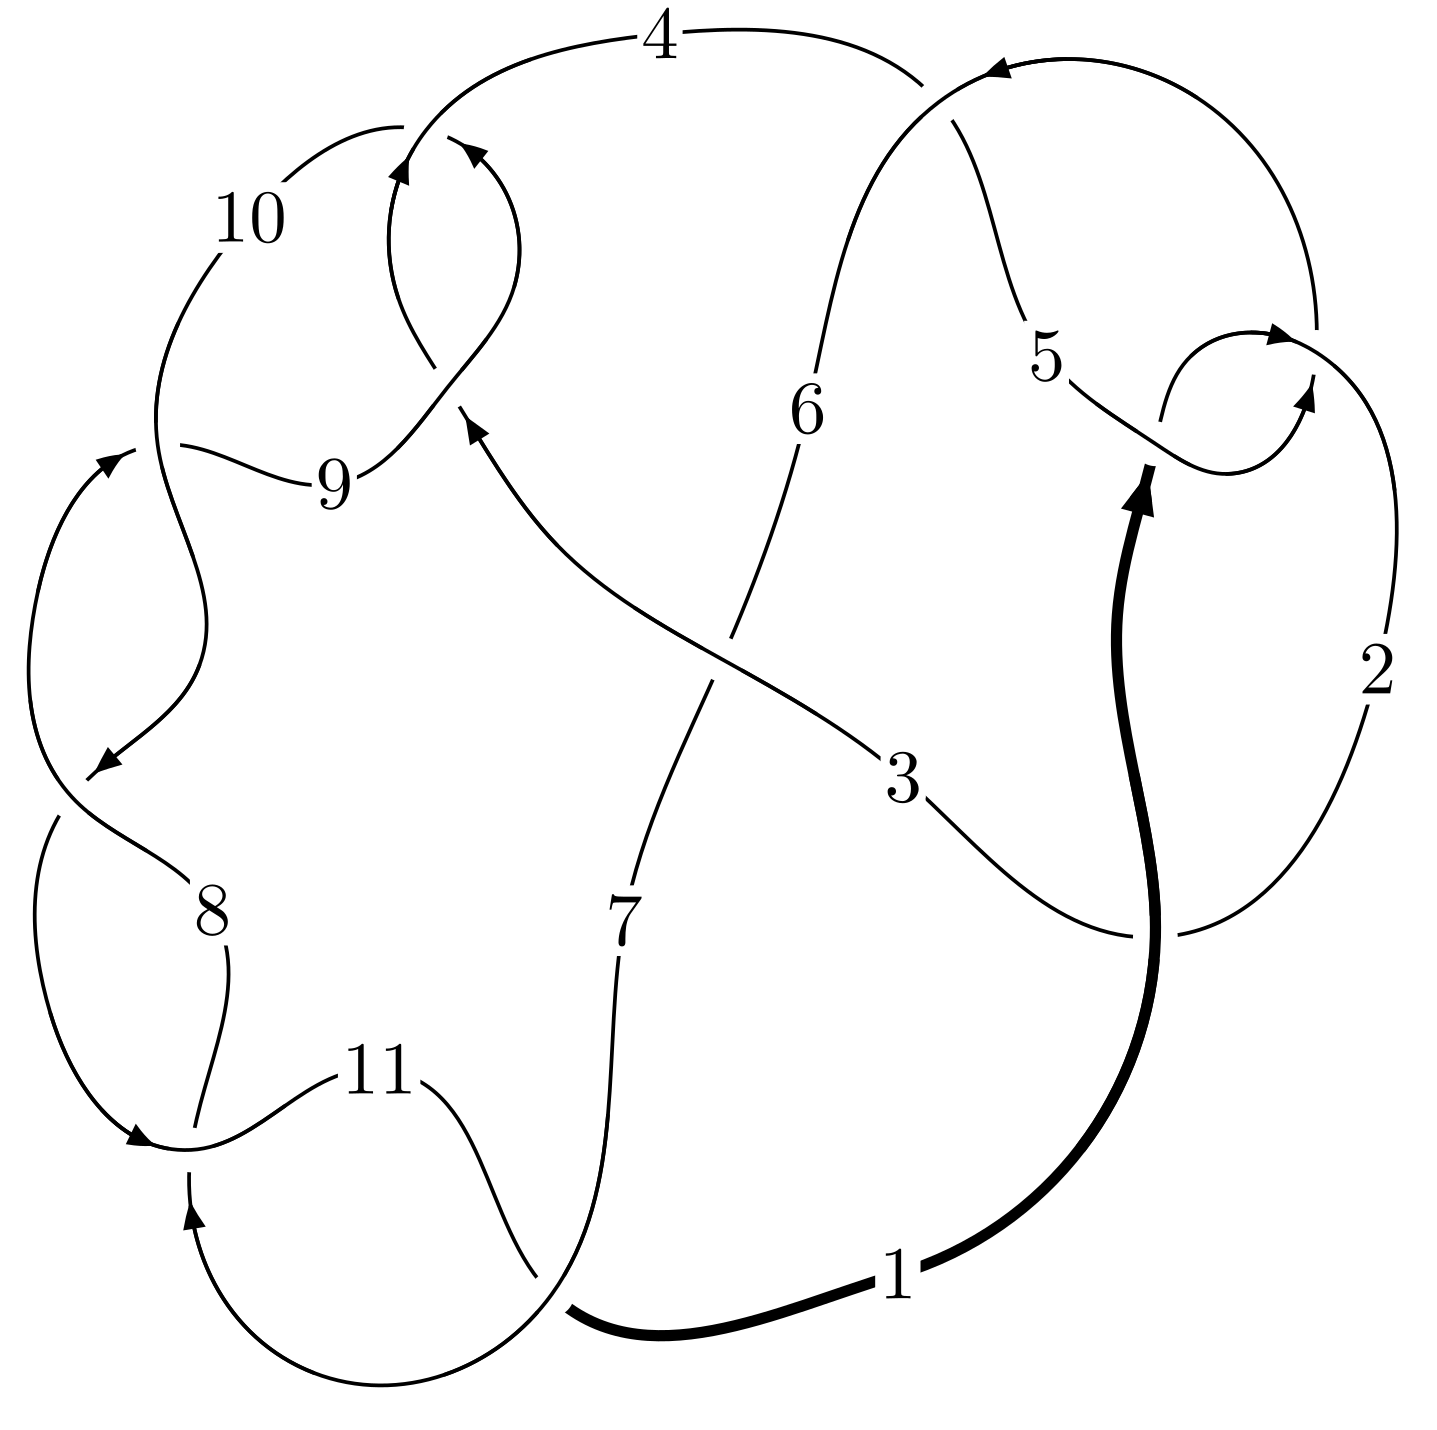
\includegraphics[width=112pt]{../../../GIT/diagram.site/Diagrams/png/344_11a_95.png}\\
\ \ \ A knot diagram\footnotemark}&
\allowdisplaybreaks
\textbf{Linearized knot diagam} \\
\cline{2-2}
 &
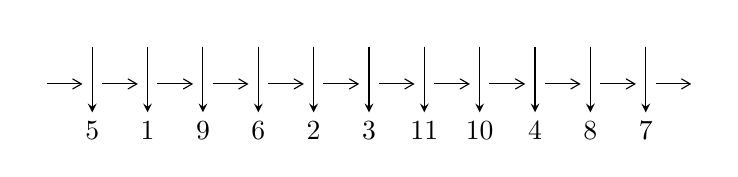
\begin{tikzpicture}[x=20pt, y=17pt]
	% nodes
	\node (C0) at (0, 0) {};
	\node (C1) at (1, 0) {};
	\node (C1U) at (1, +1) {};
	\node (C1D) at (1, -1) {5};

	\node (C2) at (2, 0) {};
	\node (C2U) at (2, +1) {};
	\node (C2D) at (2, -1) {1};

	\node (C3) at (3, 0) {};
	\node (C3U) at (3, +1) {};
	\node (C3D) at (3, -1) {9};

	\node (C4) at (4, 0) {};
	\node (C4U) at (4, +1) {};
	\node (C4D) at (4, -1) {6};

	\node (C5) at (5, 0) {};
	\node (C5U) at (5, +1) {};
	\node (C5D) at (5, -1) {2};

	\node (C6) at (6, 0) {};
	\node (C6U) at (6, +1) {};
	\node (C6D) at (6, -1) {3};

	\node (C7) at (7, 0) {};
	\node (C7U) at (7, +1) {};
	\node (C7D) at (7, -1) {11};

	\node (C8) at (8, 0) {};
	\node (C8U) at (8, +1) {};
	\node (C8D) at (8, -1) {10};

	\node (C9) at (9, 0) {};
	\node (C9U) at (9, +1) {};
	\node (C9D) at (9, -1) {4};

	\node (C10) at (10, 0) {};
	\node (C10U) at (10, +1) {};
	\node (C10D) at (10, -1) {8};

	\node (C11) at (11, 0) {};
	\node (C11U) at (11, +1) {};
	\node (C11D) at (11, -1) {7};
	\node (C12) at (12, 0) {};

	% arrows
	\draw[->,>={angle 60}]
	(C0) edge (C1) (C1) edge (C2) (C2) edge (C3) (C3) edge (C4) (C4) edge (C5) (C5) edge (C6) (C6) edge (C7) (C7) edge (C8) (C8) edge (C9) (C9) edge (C10) (C10) edge (C11) (C11) edge (C12) ;	\draw[->,>=stealth]
	(C1U) edge (C1D) (C2U) edge (C2D) (C3U) edge (C3D) (C4U) edge (C4D) (C5U) edge (C5D) (C6U) edge (C6D) (C7U) edge (C7D) (C8U) edge (C8D) (C9U) edge (C9D) (C10U) edge (C10D) (C11U) edge (C11D) ;
	\end{tikzpicture} \\
\hhline{~~} \\& 
\textbf{Solving Sequence} \\ \cline{2-2} 
 &
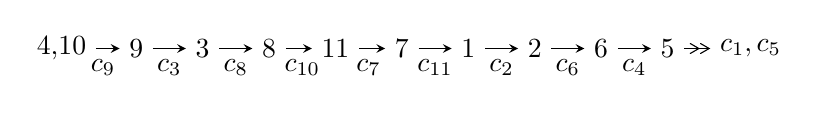
\begin{tikzpicture}[x=24pt, y=7pt]
	% node
	\node (A0) at (-1/8, 0) {4,10};
	\node (A1) at (1, 0) {9};
	\node (A2) at (2, 0) {3};
	\node (A3) at (3, 0) {8};
	\node (A4) at (4, 0) {11};
	\node (A5) at (5, 0) {7};
	\node (A6) at (6, 0) {1};
	\node (A7) at (7, 0) {2};
	\node (A8) at (8, 0) {6};
	\node (A9) at (9, 0) {5};
	\node (C1) at (1/2, -1) {$c_{9}$};
	\node (C2) at (3/2, -1) {$c_{3}$};
	\node (C3) at (5/2, -1) {$c_{8}$};
	\node (C4) at (7/2, -1) {$c_{10}$};
	\node (C5) at (9/2, -1) {$c_{7}$};
	\node (C6) at (11/2, -1) {$c_{11}$};
	\node (C7) at (13/2, -1) {$c_{2}$};
	\node (C8) at (15/2, -1) {$c_{6}$};
	\node (C9) at (17/2, -1) {$c_{4}$};
	\node (A10) at (41/4, 0) {$c_{1},c_{5}$};

	% edge
	\draw[->,>=stealth]	
	(A0) edge (A1) (A1) edge (A2) (A2) edge (A3) (A3) edge (A4) (A4) edge (A5) (A5) edge (A6) (A6) edge (A7) (A7) edge (A8) (A8) edge (A9) ;
	\draw[->>,>={angle 60}]	
	(A9) edge (A10);
\end{tikzpicture} \\ 

\end{tabular} \\

\footnotetext{
The image of knot diagram is generated by the software ``\textbf{Draw programme}" developed by Andrew Bartholomew(\url{http://www.layer8.co.uk/maths/draw/index.htm\#Running-draw}), where we modified some parts for our purpose(\url{https://github.com/CATsTAILs/LinksPainter}).
}\phantom \\ \newline 
\centering \textbf{Ideals for irreducible components\footnotemark of $X_{\text{par}}$} 
 
\begin{align*}
I^u_{1}&=\langle 
u^{36}+u^{35}+\cdots+2 u-1\rangle \\
\\
\end{align*}
\raggedright * 1 irreducible components of $\dim_{\mathbb{C}}=0$, with total 36 representations.\\
\footnotetext{All coefficients of polynomials are rational numbers. But the coefficients are sometimes approximated in decimal forms when there is not enough margin.}
\newpage
\renewcommand{\arraystretch}{1}
\centering \section*{I. $I^u_{1}= \langle u^{36}+u^{35}+\cdots+2 u-1 \rangle$}
\flushleft \textbf{(i) Arc colorings}\\
\begin{tabular}{m{7pt} m{180pt} m{7pt} m{180pt} }
\flushright $a_{4}=$&$\begin{pmatrix}0\\u\end{pmatrix}$ \\
\flushright $a_{10}=$&$\begin{pmatrix}1\\0\end{pmatrix}$ \\
\flushright $a_{9}=$&$\begin{pmatrix}1\\- u^2\end{pmatrix}$ \\
\flushright $a_{3}=$&$\begin{pmatrix}u\\- u^3+u\end{pmatrix}$ \\
\flushright $a_{8}=$&$\begin{pmatrix}- u^2+1\\- u^2\end{pmatrix}$ \\
\flushright $a_{11}=$&$\begin{pmatrix}u^4- u^2+1\\u^4\end{pmatrix}$ \\
\flushright $a_{7}=$&$\begin{pmatrix}- u^6+u^4-2 u^2+1\\- u^6- u^2\end{pmatrix}$ \\
\flushright $a_{1}=$&$\begin{pmatrix}u^8- u^6+3 u^4-2 u^2+1\\u^8+2 u^4\end{pmatrix}$ \\
\flushright $a_{2}=$&$\begin{pmatrix}- u^{19}+2 u^{17}-8 u^{15}+12 u^{13}-21 u^{11}+22 u^9-20 u^7+12 u^5-5 u^3+2 u\\- u^{19}+u^{17}-6 u^{15}+5 u^{13}-11 u^{11}+7 u^9-6 u^7+2 u^5- u^3+u\end{pmatrix}$ \\
\flushright $a_{6}=$&$\begin{pmatrix}- u^{10}+u^8-4 u^6+3 u^4-3 u^2+1\\u^{12}-2 u^{10}+4 u^8-6 u^6+3 u^4-2 u^2\end{pmatrix}$ \\
\flushright $a_{5}=$&$\begin{pmatrix}- u^{21}+2 u^{19}+\cdots+6 u^3- u\\u^{23}-3 u^{21}+\cdots+2 u^3+u\end{pmatrix}$\\ \flushright $a_{5}=$&$\begin{pmatrix}- u^{21}+2 u^{19}+\cdots+6 u^3- u\\u^{23}-3 u^{21}+\cdots+2 u^3+u\end{pmatrix}$\\&\end{tabular}
\flushleft \textbf{(ii) Obstruction class $= -1$}\\~\\
\flushleft \textbf{(iii) Cusp Shapes $= -4 u^{34}-4 u^{33}+12 u^{32}+16 u^{31}-60 u^{30}-68 u^{29}+136 u^{28}+180 u^{27}-352 u^{26}-420 u^{25}+612 u^{24}+780 u^{23}-1052 u^{22}-1232 u^{21}+1408 u^{20}+1624 u^{19}-1744 u^{18}-1804 u^{17}+1796 u^{16}+1644 u^{15}-1644 u^{14}-1232 u^{13}+1288 u^{12}+704 u^{11}-852 u^{10}-296 u^9+456 u^8+44 u^7-184 u^6+44 u^5+40 u^4-36 u^3+12 u-18$}\\~\\
\newpage\renewcommand{\arraystretch}{1}
\flushleft \textbf{(iv) u-Polynomials at the component}\newline \\
\begin{tabular}{m{50pt}|m{274pt}}
Crossings & \hspace{64pt}u-Polynomials at each crossing \\
\hline $$\begin{aligned}c_{1},c_{5}\end{aligned}$$&$\begin{aligned}
&u^{36}+u^{35}+\cdots-4 u-1
\end{aligned}$\\
\hline $$\begin{aligned}c_{2},c_{4}\end{aligned}$$&$\begin{aligned}
&u^{36}+11 u^{35}+\cdots+6 u+1
\end{aligned}$\\
\hline $$\begin{aligned}c_{3},c_{9}\end{aligned}$$&$\begin{aligned}
&u^{36}- u^{35}+\cdots-2 u-1
\end{aligned}$\\
\hline $$\begin{aligned}c_{6}\end{aligned}$$&$\begin{aligned}
&u^{36}- u^{35}+\cdots-366 u-97
\end{aligned}$\\
\hline $$\begin{aligned}c_{7},c_{8},c_{10}\\c_{11}\end{aligned}$$&$\begin{aligned}
&u^{36}+7 u^{35}+\cdots+6 u+1
\end{aligned}$\\
\hline
\end{tabular}\\~\\
\newpage\renewcommand{\arraystretch}{1}
\flushleft \textbf{(v) Riley Polynomials at the component}\newline \\
\begin{tabular}{m{50pt}|m{274pt}}
Crossings & \hspace{64pt}Riley Polynomials at each crossing \\
\hline $$\begin{aligned}c_{1},c_{5}\end{aligned}$$&$\begin{aligned}
&y^{36}-11 y^{35}+\cdots-6 y+1
\end{aligned}$\\
\hline $$\begin{aligned}c_{2},c_{4}\end{aligned}$$&$\begin{aligned}
&y^{36}+29 y^{35}+\cdots-62 y+1
\end{aligned}$\\
\hline $$\begin{aligned}c_{3},c_{9}\end{aligned}$$&$\begin{aligned}
&y^{36}-7 y^{35}+\cdots-6 y+1
\end{aligned}$\\
\hline $$\begin{aligned}c_{6}\end{aligned}$$&$\begin{aligned}
&y^{36}+17 y^{35}+\cdots-13870 y+9409
\end{aligned}$\\
\hline $$\begin{aligned}c_{7},c_{8},c_{10}\\c_{11}\end{aligned}$$&$\begin{aligned}
&y^{36}+45 y^{35}+\cdots-14 y+1
\end{aligned}$\\
\hline
\end{tabular}\\~\\
\newpage\flushleft \textbf{(vi) Complex Volumes and Cusp Shapes}
$$\begin{array}{c|c|c}  
\text{Solutions to }I^u_{1}& \I (\text{vol} + \sqrt{-1}CS) & \text{Cusp shape}\\
 \hline 
\begin{aligned}
u &= \phantom{-}0.855468 + 0.478503 I\end{aligned}
 & -1.79064 - 4.12069 I & -14.4783 + 7.6804 I \\ \hline\begin{aligned}
u &= \phantom{-}0.855468 - 0.478503 I\end{aligned}
 & -1.79064 + 4.12069 I & -14.4783 - 7.6804 I \\ \hline\begin{aligned}
u &= -0.885209 + 0.588905 I\end{aligned}
 & \phantom{-}4.26116 + 3.38021 I & -6.36942 - 4.06127 I \\ \hline\begin{aligned}
u &= -0.885209 - 0.588905 I\end{aligned}
 & \phantom{-}4.26116 - 3.38021 I & -6.36942 + 4.06127 I \\ \hline\begin{aligned}
u &= \phantom{-}0.910885 + 0.568898 I\end{aligned}
 & \phantom{-}3.52152 - 9.06176 I & -8.19420 + 9.30306 I \\ \hline\begin{aligned}
u &= \phantom{-}0.910885 - 0.568898 I\end{aligned}
 & \phantom{-}3.52152 + 9.06176 I & -8.19420 - 9.30306 I \\ \hline\begin{aligned}
u &= -0.612613 + 0.694030 I\end{aligned}
 & \phantom{-}5.14913 + 1.38552 I & -3.93165 - 2.60854 I \\ \hline\begin{aligned}
u &= -0.612613 - 0.694030 I\end{aligned}
 & \phantom{-}5.14913 - 1.38552 I & -3.93165 + 2.60854 I \\ \hline\begin{aligned}
u &= -0.740711 + 0.536049 I\end{aligned}
 & \phantom{-}1.42228 + 2.05301 I & -4.86610 - 4.82950 I \\ \hline\begin{aligned}
u &= -0.740711 - 0.536049 I\end{aligned}
 & \phantom{-}1.42228 - 2.05301 I & -4.86610 + 4.82950 I \\ \hline\begin{aligned}
u &= \phantom{-}0.568507 + 0.699594 I\end{aligned}
 & \phantom{-}4.63406 + 4.35057 I & -4.96741 - 3.00405 I \\ \hline\begin{aligned}
u &= \phantom{-}0.568507 - 0.699594 I\end{aligned}
 & \phantom{-}4.63406 - 4.35057 I & -4.96741 + 3.00405 I \\ \hline\begin{aligned}
u &= -0.882589 + 0.153471 I\end{aligned}
 & -0.44906 + 4.79281 I & -14.2901 - 6.9019 I \\ \hline\begin{aligned}
u &= -0.882589 - 0.153471 I\end{aligned}
 & -0.44906 - 4.79281 I & -14.2901 + 6.9019 I \\ \hline\begin{aligned}
u &= \phantom{-}0.835861 + 0.225802 I\end{aligned}
 & -0.001943 + 0.306901 I & -12.89345 + 1.58755 I \\ \hline\begin{aligned}
u &= \phantom{-}0.835861 - 0.225802 I\end{aligned}
 & -0.001943 - 0.306901 I & -12.89345 - 1.58755 I \\ \hline\begin{aligned}
u &= -0.854609\phantom{ +0.000000I}\end{aligned}
 & -4.25142\phantom{ +0.000000I} & -21.1240\phantom{ +0.000000I} \\ \hline\begin{aligned}
u &= -0.905500 + 0.888140 I\end{aligned}
 & \phantom{-}6.73510 + 0.05242 I & -9.91031 + 1.11538 I \\ \hline\begin{aligned}
u &= -0.905500 - 0.888140 I\end{aligned}
 & \phantom{-}6.73510 - 0.05242 I & -9.91031 - 1.11538 I \\ \hline\begin{aligned}
u &= -0.942056 + 0.872713 I\end{aligned}
 & \phantom{-}6.61933 + 6.45885 I & -10.23279 - 5.88059 I \\ \hline\begin{aligned}
u &= -0.942056 - 0.872713 I\end{aligned}
 & \phantom{-}6.61933 - 6.45885 I & -10.23279 + 5.88059 I \\ \hline\begin{aligned}
u &= \phantom{-}0.929633 + 0.892365 I\end{aligned}
 & \phantom{-}10.03410 - 3.29411 I & -3.98637 + 2.43304 I \\ \hline\begin{aligned}
u &= \phantom{-}0.929633 - 0.892365 I\end{aligned}
 & \phantom{-}10.03410 + 3.29411 I & -3.98637 - 2.43304 I \\ \hline\begin{aligned}
u &= -0.901015 + 0.922180 I\end{aligned}
 & \phantom{-}13.3053 - 5.0936 I & -5.21713 + 2.79441 I \\ \hline\begin{aligned}
u &= -0.901015 - 0.922180 I\end{aligned}
 & \phantom{-}13.3053 + 5.0936 I & -5.21713 - 2.79441 I \\ \hline\begin{aligned}
u &= \phantom{-}0.909275 + 0.920439 I\end{aligned}
 & \phantom{-}14.07570 - 0.94615 I & -3.96028 + 2.12397 I \\ \hline\begin{aligned}
u &= \phantom{-}0.909275 - 0.920439 I\end{aligned}
 & \phantom{-}14.07570 + 0.94615 I & -3.96028 - 2.12397 I \\ \hline\begin{aligned}
u &= \phantom{-}0.962084 + 0.893022 I\end{aligned}
 & \phantom{-}13.9035 - 5.7329 I & -4.26372 + 2.53612 I \\ \hline\begin{aligned}
u &= \phantom{-}0.962084 - 0.893022 I\end{aligned}
 & \phantom{-}13.9035 + 5.7329 I & -4.26372 - 2.53612 I \\ \hline\begin{aligned}
u &= -0.967629 + 0.887890 I\end{aligned}
 & \phantom{-}13.0885 + 11.7607 I & -5.64793 - 7.43079 I\\
 \hline 
 \end{array}$$\newpage$$\begin{array}{c|c|c}  
\text{Solutions to }I^u_{1}& \I (\text{vol} + \sqrt{-1}CS) & \text{Cusp shape}\\
 \hline 
\begin{aligned}
u &= -0.967629 - 0.887890 I\end{aligned}
 & \phantom{-}13.0885 - 11.7607 I & -5.64793 + 7.43079 I \\ \hline\begin{aligned}
u &= \phantom{-}0.484510 + 0.469460 I\end{aligned}
 & -0.731880 + 0.351895 I & -10.65376 - 0.66893 I \\ \hline\begin{aligned}
u &= \phantom{-}0.484510 - 0.469460 I\end{aligned}
 & -0.731880 - 0.351895 I & -10.65376 + 0.66893 I \\ \hline\begin{aligned}
u &= \phantom{-}0.043246 + 0.549053 I\end{aligned}
 & \phantom{-}2.46542 - 2.71564 I & -4.42006 + 3.22989 I \\ \hline\begin{aligned}
u &= \phantom{-}0.043246 - 0.549053 I\end{aligned}
 & \phantom{-}2.46542 + 2.71564 I & -4.42006 - 3.22989 I \\ \hline\begin{aligned}
u &= \phantom{-}0.530314\phantom{ +0.000000I}\end{aligned}
 & -0.709168\phantom{ +0.000000I} & -14.3100\phantom{ +0.000000I}\\
 \hline 
 \end{array}$$\newpage
\newpage\renewcommand{\arraystretch}{1}
\centering \section*{ II. u-Polynomials}
\begin{tabular}{m{50pt}|m{274pt}}
Crossings & \hspace{64pt}u-Polynomials at each crossing \\
\hline $$\begin{aligned}c_{1},c_{5}\end{aligned}$$&$\begin{aligned}
&u^{36}+u^{35}+\cdots-4 u-1
\end{aligned}$\\
\hline $$\begin{aligned}c_{2},c_{4}\end{aligned}$$&$\begin{aligned}
&u^{36}+11 u^{35}+\cdots+6 u+1
\end{aligned}$\\
\hline $$\begin{aligned}c_{3},c_{9}\end{aligned}$$&$\begin{aligned}
&u^{36}- u^{35}+\cdots-2 u-1
\end{aligned}$\\
\hline $$\begin{aligned}c_{6}\end{aligned}$$&$\begin{aligned}
&u^{36}- u^{35}+\cdots-366 u-97
\end{aligned}$\\
\hline $$\begin{aligned}c_{7},c_{8},c_{10}\\c_{11}\end{aligned}$$&$\begin{aligned}
&u^{36}+7 u^{35}+\cdots+6 u+1
\end{aligned}$\\
\hline
\end{tabular}\newpage\renewcommand{\arraystretch}{1}
\centering \section*{ III. Riley Polynomials}
\begin{tabular}{m{50pt}|m{274pt}}
Crossings & \hspace{64pt}Riley Polynomials at each crossing \\
\hline $$\begin{aligned}c_{1},c_{5}\end{aligned}$$&$\begin{aligned}
&y^{36}-11 y^{35}+\cdots-6 y+1
\end{aligned}$\\
\hline $$\begin{aligned}c_{2},c_{4}\end{aligned}$$&$\begin{aligned}
&y^{36}+29 y^{35}+\cdots-62 y+1
\end{aligned}$\\
\hline $$\begin{aligned}c_{3},c_{9}\end{aligned}$$&$\begin{aligned}
&y^{36}-7 y^{35}+\cdots-6 y+1
\end{aligned}$\\
\hline $$\begin{aligned}c_{6}\end{aligned}$$&$\begin{aligned}
&y^{36}+17 y^{35}+\cdots-13870 y+9409
\end{aligned}$\\
\hline $$\begin{aligned}c_{7},c_{8},c_{10}\\c_{11}\end{aligned}$$&$\begin{aligned}
&y^{36}+45 y^{35}+\cdots-14 y+1
\end{aligned}$\\
\hline
\end{tabular}
\vskip 2pc
\end{document}